
\documentclass[11pt,a4paper,oneside]{report}

\synctex=1

\usepackage{pslatex,palatino,avant,graphicx,color}
\usepackage[margin=2cm]{geometry}

\usepackage{mathptmx}       % selects Times Roman as basic font

\usepackage{helvet}         % selects Helvetica as sans-serif font
\usepackage{courier}        % selects Courier as typewriter font
\usepackage{type1cm}        % activate if the above 3 fonts are
                            % not available on your system

\usepackage{makeidx}         % allows index generation
\usepackage{graphicx}        % standard LaTeX graphics tool
                             % when including figure files
\usepackage{multicol}        % used for the two-column index
\usepackage{multirow}
\usepackage{booktabs}

\usepackage[bottom]{footmisc}% places footnotes at page bottom

\usepackage[utf8]{inputenc}
\inputencoding{utf8}


%\usepackage[round]{natbib}
\usepackage[square,sort]{natbib}
\bibliographystyle{unsrtnat}


\usepackage[utf8]{inputenc}
\usepackage[english]{babel}

\usepackage{longtable}
\usepackage{pdflscape}

%for formula references
\usepackage{amsmath}
\newtheorem{mydef}{Definition}

\usepackage{changes}
%triangledown
\usepackage{latexsym}
\usepackage{amssymb}
\usepackage{amsfonts}


%langle
\usepackage{scalerel}
\usepackage{graphicx}

%cite

%\usepackage[USenglish]{babel}
%\usepackage[nodayofweek,level]{datetime}
%\newcommand{\mydate}{\formatdate{4}{11}{2014}}

\makeindex

\begin{document}
\title{On Selecting Heuristics Functions for Domain-Independent Planning.}
\providecommand{\keywords}[1]{\textbf{keywords} #1}
\author{Student: Marvin Abisrror Zarate\\ Advisor: Levi Lelis \\
Departamento de Informática \\Universidade Federal de Vicosa \\Viçosa, Brazil}

\date{\color{black}July 2015}
\maketitle

\section{Introduction}
\label{sec:1}
Selecting a subset of heuristics functions in order to solve Domain-Indepentent Planning problems using A* search algorithm is an approach that selects the most promising heuristics from a bunch of heuristics that were generated based on the concepts of reducing the search tree and combination of primitive heuristics \citep{BarleySantiagoOver}
\\
This project is concerned with cost-optimal state-space planning using the A* algorithm and finding strategies to make the A* search algorithm finishes quickly is our main aim. The approach can be applied for solving optimal domain problems in the Fast-Downward Planner. A few of these are: Elevators opt08 and opt11, Floortile opt11, Nomystery opt11, etc.
\\
The approach we choose to select the most promising heuristics is Deterministic and is based on the ranking of heuristics according the number of nodes generated running the Stratification Sampling algorithm (SS). The SS system (Lelis  2013) is a Stocastic approach that produces accurate results predicting the number of nodes expanded by IDA*. Nevertheless, we are aware that SS can not be easily adapted to A* because A*'s duplicate pruning makes it very difficult to predict how many nodes will occur at depth \textit{\textbf{d}} of A* search tree (the tree of nodes expanded by A*). That is the principal reason why we decided to create the concept of \textit{regret} which is the cost from not to choose the heuristic that generates the lowest number of nodes generated or the best heuristic. If the \textit{regret} for one heuristic is very close to zero when running A* then it is a promising heuristic.

\newpage

This project is concerned with cost-optimal state-space planning using the A* algorithm \citep{hart1968formal}. We assume that a pool $\zeta$, of hundreds or even thousands of heuristics  is available, and that the final heuristic used to guide A*, $h\textsubscript{max}$, will be defined as the maximum over a subset $\zeta\sp{\prime}$ of those heuristics (\textit{$h\textsubscript{max}(s, \zeta\sp{\prime})$} =  $\max_{h\epsilon \zeta\sp{\prime}}h(s)$). The choice of the subset $\zeta\sp{\prime}$ can greatly affect the efficiency of A*. For a given size \textit{N} and planning task $\triangledown$, a subset containing \textit{N} heuristics from $\zeta$ is optimal if no other subset containing \textit{N} heuristics from $\zeta$ result in A* expanding fewer nodes when solving $\triangledown$ (in the worst case-see the formal definition below).
\newline

The first contribution of this research is to show that the problem of finding the optimal subset of $\zeta$ of size \textit{N} for a given problem task is supermodular, and therefore a greedy algorithm, which we call Greedy Heuristic Selection (GHS), that selects heuristics from $\zeta$ one at a time is guaranteed to produce a subset $\zeta\sp{\prime}$ such that the number of nodes expanded by A* is no more than approximately 1.36 times optimal. An optimization procedure which is similar to ours is presented by citaRayner, but their procedure maximizes the average heuristic value. By contrast, GHS minimizes the search three size.  GHS requires a prediction of the number of nodes expanded by A* using any given subset. Although there are methods for accurately predicting the number of nodes expanded by Iterative Deepening-A* \citep{Korf85ida} (IDA*) (e.g the SS system \citep{lelis2013predicting}), these methods can't be easily adapted to A* because A*'s duplicate pruning makes it very difficult to predict how many nodes will occur at depth \textit{d} of A*'s search tree (the tree of nodes expanded by A*). In this research we use a method for predicting the size of A*'s search tree which is based on the prediction method presented by BarleySantiagoOver
\newline
The second contribution of this research is an emperical evaluation of GHS in optimal domain-independent planning problems. Namely, there are experiments in the 2011 International Planning Competition (IPC) where the subset chosen by the GHS can be far superior, in terms of coverage, to defining $h\textsubscript{max}$ over the entire collection $\zeta$ and competitive with other state-of-the-art methods.
\newline
The system most similar to GHS is RIDA* also selects a subset from a pool of heuristics to guide the A* search. In RIDA* this is done by starting with an empty subset and trying all combinations of size one before trying the combinations of size two and so on. RIDA* stops after evaluating a fixed number of subsets. While RIDA* is able to evaluate a set of heuristics with tens of elements, GHS is able to evaluate a set of heuristics with thousand of elements.
\newline
\section{Background}
An \textit{SAS$\sp{+}$} \citep{backstrom1995complexity} is a 4-tuple 
$\triangledown$ = ${\langle \nu N O \rangle}$


We use as experiments the competitions domains problems from the fast-downward benchmarks. The planner contains satisficing and optimization track problems, the satisficing problem are so hard to work and also is difficicult to found an optimal solutions, so they could be used to research because we pretend to predict the number of nodes expanded in the tree but we won't found an optimal solutions and also it would skip our analysis using consistent heuristics. In this research we will use the problems that require optimization in order to test our approach. 

\subsection{Problem Domains}
Two of the optimal domain problems we have worked are barman and parking. The block domain contains easy instances that are very good to test our approach quickly.

\subsubsection{Barman}
This domain was created for the \textit{International Planning Competition (IPC)} in \textit{2011}. In this domain there is a robot barman that manipulates drink dispensers, glasses and shaker. The goal is to find a plan of the robot's actions that serves a desired set of drinks.

\subsubsection{Parking}
This domain was created for learning track \textit{IPC-2008}. This domain involves parking cars on a street with N curb locations, and where cars can be double-parked but not triple-parked. The goal is to find a plan to move from one configuration of parked cars to another configuration, by driving cars from one curb location to another. 

\subsubsection{Blocks World}
This domain had origin in the \textit{IPC-2000}. This domain consists of a set of blocks, a table and a robot hand. The blocks can be on top of other blocks or on the table; a block that has nothing on it is clear; and the robot hand can hold one block or be empty. The goal is to find a plan to move from one configuration of blocks to another. The problem probBLOCKS-4-0 is going to be our instance that will be used to explain our results in this Project. We chosen that because is a simple problem that can be resolved in less than few seconds and also contains the characteristics of duplicate nodes.

\section{Problem Formulation}
Let the \textit{underlying search tree} (\textit{UST}) be the full brute-force tree created from a connected, undirected and implicitly defined \textit{underlying search graph} (\textit{USG}) describing a state space. Some search algoritms expand a subtree of the \textit{UST} while searching for a solution (e.g., a portion of the \textit{UST} might not be expanded due to heuristic guidence.); we call this subtree the \textit{expanded search tree} (\textit{UST}). In this paper we want to estimate the size of the subgraph expanded by an algorithm searching the (\textit{USG}); we call this subgraph the \textit{expanded search graph} (\textit{ESG})

\begin{mydef}
\textit{(Canonical and Duplicate Nodes). A node n in the UST is called a duplicate node if there exists another node n' in the UST such that state(s) $=$ state(n') and n' $<$  n. A node that is not duplicate is called a canonical node.}
\end{mydef}

We define three graphs: The first one is the graph generated by dijkstra algorithm (\textit{subtree of the UST}), which contains the tree without duplicate nodes. The second is the Brute Force Search tree generated by the Stratified Sampling algorithm which generate duplicate nodes and the last one is the tree generated by A* using a consistent heuristic which is also the tree we want to predict.\newline

Formally, Let \textit{G = (N, E)} be a  graph representing an expanded search graph (ESG) of  each graph explained above where \textit{N} is its set of states and  for each:
\[  {n \in  N / op(n) =  {op_i|(n, n_i)}  \in E }  \]

 is its set of operators. We use the words edges and operators interchangeably. The prediction is to estimate the size of \textit{N} without fully generate the ESG from A*.

\section{Predicting the size of the Search Graph}
We now explain how we pretend to achieve the prediction of the number of  nodes expanded by A*.\newline

\subsection{Dijkstra Algorithm}
Dijkstra Algorithm is an uninformed search algorithm. In our cost function the value of \textbf{\textit{h}} is \textbf{\textit{0}} for all the nodes of the search tree and the value \textbf{\textit{g}} increase according to the level of the tree. It means that there is no guide to search the goal, in each iteratation the nodes from a level expand blindly according to the value of the level  up to find the goal node. We collect the total number of nodes expanded by level without prunning. So, for our exemple in the level \textbf{\textit{0}} we have one node which is initial state, in the level \textbf{\textit{1}} we have \textbf{\textit{4}} nodes, level \textbf{\textit{2}} contains \textbf{\textit{12}} nodes, etc. This information is collected in the planner executing A* using the dijkstra heuristic which assign the value zero for all the nodes in the search tree. 

\begin{figure}[htb]
\begin{center}
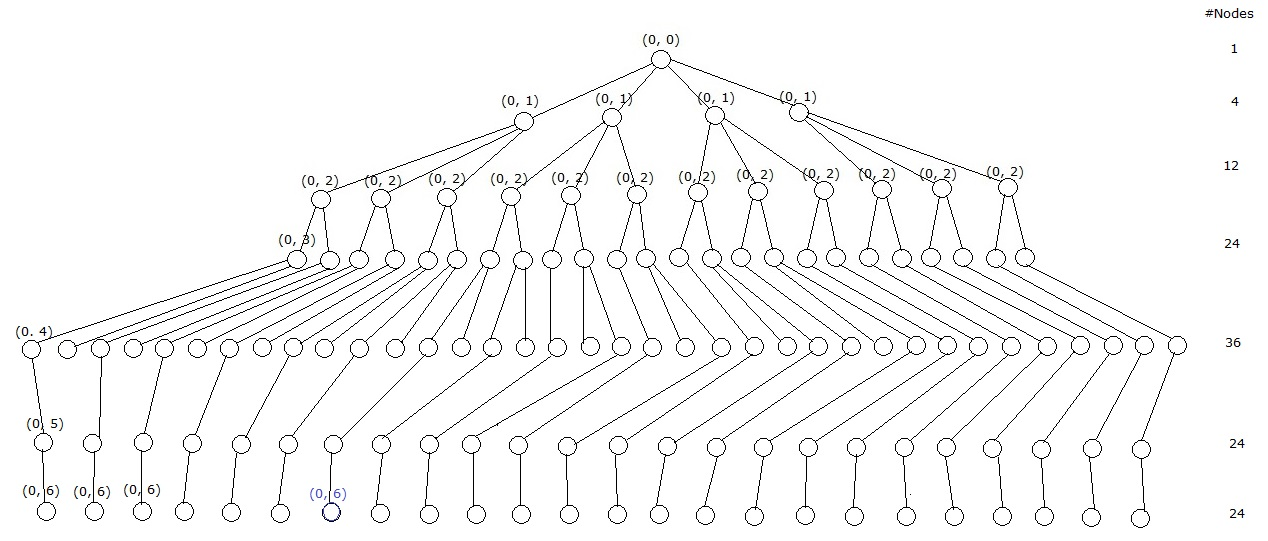
\includegraphics[width=12cm]{./image/dijkstra}
\caption{The par value (\textbf{\textit{h}}, \textbf{\textit{g}}) represent the heuristic value \textbf{\textit{h}} and the cost to go from the start state to the current node \textbf{\textit{g}}. The tree generated by Dijkstra Search Algorithm to the problem of blocks worlds probBLOCKS-4-0.}
\label{fig:dijkstraTreeInconsistent}
\end{center}
\end{figure}

In the Figure~\ref{fig:dijkstraTreeInconsistent} are showed the total number of nodes expanded by level and also how the tree is distributed.\newline

We also, present the Table~\ref{table:tabledijstraExpandedByLevel} which explain the distribution of nodes expanded by level during dijkstra search algorithm.\newline

\footnotesize  % Switch from 12pt to 11pt; otherwise, table won't fit
\setlength\LTleft{100pt}            % default: \fill
\setlength\LTright{200pt}           % default: \fill
\begin{longtable}{@{\extracolsep{\fill}} lll @{}} %\begin{tabular}{|c|c|}
\hline
\textit{Level} && \#Nodes expanded \\ \hline
0       && 1                \\ \hline
1       && 4                \\ \hline
2       && 12               \\ \hline
3       && 24               \\ \hline
4       && 36               \\ \hline
5       && 24               \\ \hline
6       && 24               \\ \hline
\caption{Number of nodes expanded by \textit{Level} using Dijkstra algorithm.}
\label{table:tabledijstraExpandedByLevel}
\end{longtable}

\subsection{\textit{f-value} Distribution using Dijkstra and collecting \textit{f-value} with consistent heuristic - Assumption }
In order to keep the data consistent and validate the process of the prediction we make assumptions about what we expect to obtain, for example we make comparison between \textit{f-value} distributions generated by two algorithms with the objective to see which algorithm is superior and fits fits well to our approach.\newline

\begin{figure}[htb]
\begin{center}
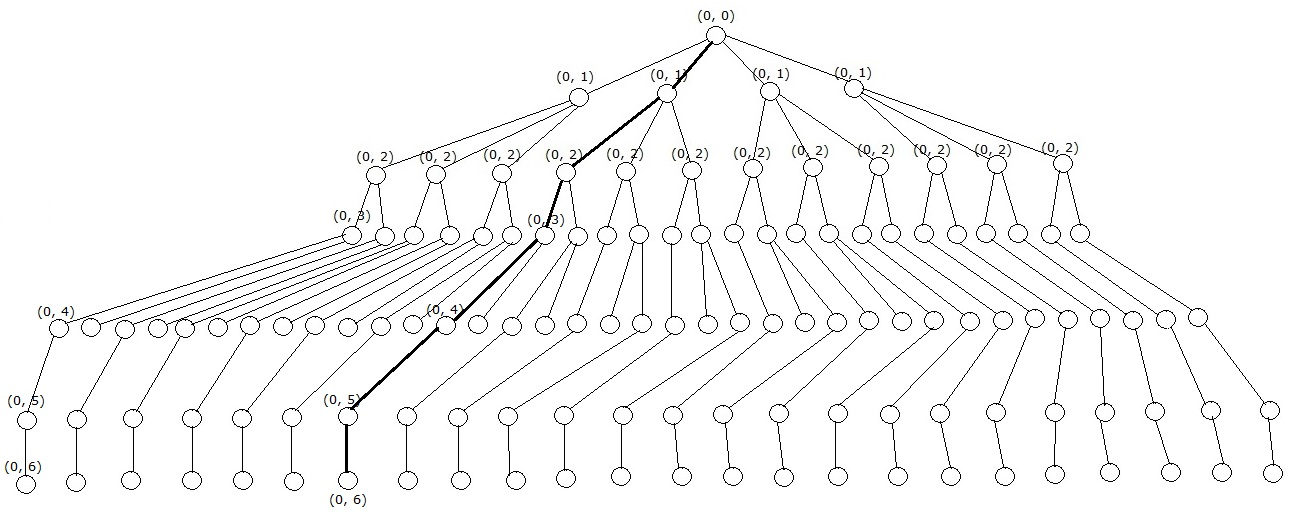
\includegraphics[width=12cm]{./image/dijkstraCollecting}
\caption{The tree generated by Dijkstra Search Algorithm and the solution route expressed by bold solid line. }
\label{fig:dijkstraTreeConsistentHeuristic}
\end{center}
\end{figure}

Starting with our assumptions we present the distribution of \textit{f-values} in the tree generated by dijkstra, but collecting the \textit{f-values} using a consistent heuristic.

The search tree generated by Dijkstra Search Algorithm expand each node blindly with heuristic value zero. In the Figure \ref{fig:dijkstraTreeConsistentHeuristic} the solid line represents the connection from the parent nodes to their childs nodes. Each node is represented with the par \textbf{\textit{(h, g)}} which represent the heuristic value \textbf{\textit{h}} and the cost to go from the origin node to the current node \textbf{\textit{g}}.\newline 

Dijkstra Algorithm iteratively expand each node in each level up to found the solution. The initial node is given by \textbf{\textit{(0, 0)}} and is located at level \textbf{\textit{0}} and the goal node is \textbf{\textit{(0, 6)}} and is at level \textbf{\textit{6}}. We expanded each node and collected the \textbf{\textit{f-value}} based on a consistent heuristic \textbf{\textit{h}} and the \textbf{\textit{g}} value of the node. The bold solid line represent the solution of using a consistent heuristic in the search. The route solution is given by: \textbf{\textit{(6, 0), (5, 1), (4, 2), (3, 3), (2, 4), (5, 1), (0, 6)}}\newline

We also present the table with the distribution of \textit{f-value} during dijkstra algorithm execution.
\footnotesize  % Switch from 12pt to 11pt; otherwise, table won't fit
\setlength\LTleft{100pt}            % default: \fill
\setlength\LTright{200pt}           % default: \fill
\begin{longtable}{@{\extracolsep{\fill}} llll @{}} %\begin{tabular}{|c|c|c|}
\hline
Level              & \textit{f-value} & quantity \\ \hline
0                  & 6       & 1        \\ \hline
\multirow{2}{*}{1} & 6       & 1        \\ \cline{2-3} 
                   & 8       & 3        \\ \hline
\multirow{3}{*}{2} & 6       & 1        \\ \cline{2-3} 
                   & 8       & 3        \\ \cline{2-3} 
                   & 10      & 8        \\ \hline
\multirow{4}{*}{3} & 6       & 1        \\ \cline{2-3} 
                   & 8       & 2        \\ \cline{2-3} 
                   & 10      & 6        \\ \cline{2-3} 
                   & 12      & 15       \\ \hline
\multirow{4}{*}{4} & 6       & 1        \\ \cline{2-3} 
                   & 12      & 2        \\ \cline{2-3} 
                   & 14      & 6        \\ \cline{2-3} 
                   & 16      & 15       \\ \hline
\multirow{4}{*}{5} & 6       & 1        \\ \cline{2-3} 
                   & 12      & 2        \\ \cline{2-3} 
                   & 14      & 6        \\ \cline{2-3} 
                   & 16      & 15       \\ \hline
\multirow{4}{*}{6} & 6       & 1        \\ \cline{2-3} 
                   & 14      & 2        \\ \cline{2-3} 
                   & 16      & 6        \\ \cline{2-3} 
                   & 18      & 15       \\ \hline
\caption{\textit{f-value} distribution expanding the graph using dijkstra and collecting the \textit{f-value} using a consistent heuristic.}
\label{table:tabledijkstra}
\end{longtable}

The Table \ref{table:tabledijkstra} represent the distribution of \textit{f-value} in the tree search expanded by dijkstra and using a consistent heuristic to collect the \textit{f-value}. The first column represent the level in which the node is located. The second column is the \textit{f-value} and the third column is the quantity, which represent the number of nodes in the level that have the same \textit{f-value}.
\newline

In order to make a prediction we will require the Formula~\eqref{eq:partitionFormula} on page \pageref{eq:partitionFormula}. $P_ex$ is the percentage of nodes expanded by level with \textit{f-value} \textbf{\textit{d}} less than to the threshold.

\footnotesize  % Switch from 12pt to 11pt; otherwise, table won't fit
\setlength\LTleft{100pt}            % default: \fill
\setlength\LTright{200pt}           % default: \fill
\begin{longtable}{@{\extracolsep{\fill}} llll @{}} %\begin{tabular}{|c|c|cl}
\hline
\textit{Level} &\rule{4pt}{0ex} Ni &\rule{0pt}{0ex} $P_ex(s, d = 6, \textit{Level})$ \\ \hline
0     &\rule{4pt}{0ex} 1\rule{16pt}{0ex}  & 1                    \\ \hline
1     &\rule{4pt}{0ex} 4\rule{4pt}{0ex}  & 0.250                \\ \hline
2     &\rule{4pt}{0ex} 12 & 0.083                \\ \hline
3     &\rule{4pt}{0ex} 24 & 0.041                \\ \hline
4     &\rule{4pt}{0ex} 36 & 0.027                \\ \hline
5     &\rule{4pt}{0ex} 24 & 0.041                \\ \hline
6     &\rule{4pt}{0ex} 24 & 0.041                \\ \hline
\caption{\textit{f-value} distribution expanding the graph using dijkstra and collecting the \textit{f-value} using a consistent heuristic.}
\label{table:tabledijkstra}
\end{longtable}

Applying the Formula~\eqref{eq:generalFormula} on page \pageref{eq:generalFormula} we obtain the prediction.

\footnotesize  % Switch from 12pt to 11pt; otherwise, table won't fit
\setlength\LTleft{100pt}            % default: \fill
\setlength\LTright{200pt}           % default: \fill
\begin{longtable}{@{\extracolsep{\fill}} lllll @{}}
\hline
                                &\rule{4pt}{0ex} threshold &\rule{4pt}{0ex} \#nodes expanded &\rule{4pt}{0ex} Prediction \\ \hline
probBLOCKS-4-0                  &\rule{4pt}{0ex} 6         &\rule{4pt}{0ex} 7                &\rule{4pt}{0ex} 7          \\ \hline
probBLOCKS-4-1                  &\rule{4pt}{0ex} 10        &\rule{4pt}{0ex} 11               &\rule{4pt}{0ex} 11         \\ \hline
probBLOCKS-4-2                  &\rule{4pt}{0ex} 6         &\rule{4pt}{0ex} 7                &\rule{4pt}{0ex} 7          \\ \hline
probBLOCKS-5-0                  &\rule{4pt}{0ex} 12        &\rule{4pt}{0ex} 16               &\rule{4pt}{0ex} 16         \\ \hline
probBLOCKS-5-1                  &\rule{4pt}{0ex} 10        &\rule{4pt}{0ex} 14               &\rule{4pt}{0ex} 14         \\ \hline
probBLOCKS-5-2                  &\rule{4pt}{0ex} 16        &\rule{4pt}{0ex} 29               &\rule{4pt}{0ex} 29         \\ \hline
probBLOCKS-6-0                  &\rule{4pt}{0ex} 12        &\rule{4pt}{0ex} 13               &\rule{4pt}{0ex} 13         \\ \hline
probBLOCKS-6-1                  &\rule{4pt}{0ex} 10        &\rule{4pt}{0ex} 11               &\rule{4pt}{0ex} 11         \\ \hline
\multirow{3}{*}{probBLOCKS-6-2} &\rule{4pt}{0ex} 18        &\rule{4pt}{0ex} 44               &\rule{4pt}{0ex} 44         \\ \cline{2-4} 
                                &\rule{4pt}{0ex} 19        &\rule{4pt}{0ex} 97               &\rule{4pt}{0ex} 97         \\ \cline{2-4} 
                                &\rule{4pt}{0ex} 20        &\rule{4pt}{0ex} 399              &\rule{4pt}{0ex} 399        \\ \hline
\multirow{4}{*}{probBLOCKS-7-0} &\rule{4pt}{0ex} 17        &\rule{4pt}{0ex} 8                &\rule{4pt}{0ex} 8          \\ \cline{2-4} 
                                &\rule{4pt}{0ex} 18        &\rule{4pt}{0ex} 30               &\rule{4pt}{0ex} 30         \\ \cline{2-4} 
                                &\rule{4pt}{0ex} 19        &\rule{4pt}{0ex} 35               &\rule{4pt}{0ex} 35         \\ \cline{2-4} 
                                &\rule{4pt}{0ex} 20        &\rule{4pt}{0ex} 243              &\rule{4pt}{0ex} 243        \\ \hline
\caption{Prediction of the number of nodes expanded by A* for the first 10 blocks world domain problems.}
\label{table:predictionDijkstra}
\end{longtable}

The Table \ref{table:predictionDijkstra} contains four columns: In the first column we have the blocks world domain problems chosen from fast-downward benchmark. We chosen 10 problems, as well as the number of the problem increases it turns more complex in terms of duplicate and expansions nodes. The second column in the threshold which represent the branches where the nodes are expanded. The third column is the number of nodes expanded by A*  in each threshold, and the last one column is the prediction.\newline

The results in the Table \ref{table:predictionDijkstra} are 100\% accurate, and this predictions are the expected, because we are testing with the same data the two terms of the prediction formula~\eqref{eq:generalFormula}. 

\subsection{\textit{f-value} Distribution using DFS - Assumption }
We have an assumption that if the distribution of the \textit{f-values} of the tree generated by dijkstra have similar structure to the distribution of the \textit{f-values} generated by Depth First Search (DFS). It would mean that the prediction using the number of nodes expanded by level with dijkstra will generate accurate values conforme to the number of nodes by \textit{f-value} generated by A*.\newline

Our assumption about the similarity of the \textit{f-value} distribution of Dijkstra and Depth First Search was tested with the same problem mentioned above obtaining the following behaviors: The \textit{f-value} distribution of Dijkstra was quickly elaborated, three steps were necesary, first the nodes expansions, the collection of the \textit{f-value} of the nodes and then the generation of the \textit{f-value} distribution file. Nevertheless, DFS last approximately less than 5 seconds to expand all the nodes and generate the \textit{f-value} which make sense because it expands just 2581 nodes. For other instances for example the probBLOCKS-6-2 just expand the nodes takes approximitely 6 minutes.\newline

So, try to generate the \textit{f-value} distribution is expensive in computational time because expand nodes the way how DFS expand the nodes is a iterative task that could take much time. So we are going to present the distribution obtained from probBLOCKS-4-0. We found that the nodes \textbf{\textit{(6, 0), (5, 1), (4, 2), (3, 3), (2, 4), (5, 1), (0, 6)}} were expanded in the same way as expanded by dijkstra algorithm, see the Table~\ref{table:tabledijkstra}  on page ~\pageref{table:tabledijkstra}. It means that the distribution of \textit{f-value} equal to 6 in each level generated by DFS is the same as the \textit{f-value} distribution with \textit{f-value} equal to 6 in each level generated by Dijkstra.\newline

According to our expience testing DFS, it could take much time to execute one instance if we set the depth of the search greater than the \textit{f-value} we are going to produce prediction. Then, after analyze the consistent heuristic we are using we set up the depth to be equal to the initial heuristic value. In this way for the problem probBLOCKS-5-0 the depth is going to be \textbf{\textit{6}}.

\footnotesize  % Switch from 12pt to 11pt; otherwise, table won't fit
\setlength\LTleft{100pt}            % default: \fill
\setlength\LTright{200pt}           % default: \fill
\begin{longtable}{@{\extracolsep{\fill}} llll @{}}
\hline

Level               & \textit{f-value} & quantity \\ \hline
0                   & 6       & 1        \\ \hline
\multirow{2}{*}{1}  & 6       & 1        \\ \cline{2-3} 
                    & 8       & 3        \\ \hline
\multirow{3}{*}{2}  & 6       & 1        \\ \cline{2-3} 
                    & 8       & 7        \\ \cline{2-3} 
                    & 10      & 8        \\ \hline
\multirow{4}{*}{3}  & 6       & 1        \\ \cline{2-3} 
                    & 8       & 9        \\ \cline{2-3} 
                    & 10      & 27       \\ \cline{2-3} 
                    & 12      & 15       \\ \hline
\multirow{5}{*}{4}  & 6       & 1        \\ \cline{2-3} 
                    & 8       & 11       \\ \cline{2-3} 
                    & 10      & 59       \\ \cline{2-3} 
                    & 12      & 88       \\ \cline{2-3} 
                    & 14      & 25       \\ \hline
\multirow{6}{*}{5}  & 6       & 1        \\ \cline{2-3} 
                    & 8       & 12       \\ \cline{2-3} 
                    & 10      & 79       \\ \cline{2-3} 
                    & 12      & 239      \\ \cline{2-3} 
                    & 14      & 186      \\ \cline{2-3} 
                    & 16      & 15       \\ \hline
\multirow{7}{*}{6}  & 6       & 1        \\ \cline{2-3} 
                    & 8       & 13       \\ \cline{2-3} 
                    & 10      & 103      \\ \cline{2-3} 
                    & 12      & 507      \\ \cline{2-3} 
                    & 14      & 832      \\ \cline{2-3} 
                    & 16      & 321      \\ \cline{2-3} 
                    & 18      & 15       \\ \hline
\caption{\textit{f-value} distribution expanding the graph using depth first search and collecting the \textit{f-value} using a consistent heuristic and threshold equal to the initial heuristic value.}
\label{table:tabledfs}
\end{longtable}

The Table \ref{table:tabledfs} represent the distribution of \textit{f-value} in the tree search expanded by depth first search using a consistent heuristic and threshold twice the initial heuristic value. Depth first search found seven nodes with \textit{f-value} equal to six in the levels \textbf{\textit{0, 1, 2, 3, 4, 5}}, and  \textbf{\textit{6}} which are the same distribution of \textit{f-value} equal to six  in Table \ref{table:tabledijkstra} on page \pageref{table:tabledijkstra}.\newline


This result encourage to continue with our research, because the distribution of dijkstra is more quickly to obtain and also make prediction over the distribution in comparison with the depth first search tree generated that is more expensive to obtain.\newline


\footnotesize  % Switch from 12pt to 11pt; otherwise, table won't fit
\setlength\LTleft{100pt}            % default: \fill
\setlength\LTright{200pt}           % default: \fill
\begin{longtable}{@{\extracolsep{\fill}} lllll @{}}
\hline
                                &\rule{4pt}{0ex} Threshold &\rule{4pt}{0ex} \#nodes expanded &\rule{4pt}{0ex} Prediction \\ \hline
probBLOCKS-4-0                  &\rule{4pt}{0ex} 6         &\rule{4pt}{0ex} 7                &\rule{4pt}{0ex} 3.54892    \\ \hline
\multirow{5}{*}{probBLOCKS-4-1} &\rule{4pt}{0ex} 4         &\rule{4pt}{0ex} 1                &\rule{4pt}{0ex} 1          \\ \cline{2-4} 
                                &\rule{4pt}{0ex} 5         &\rule{4pt}{0ex} 2                &\rule{4pt}{0ex} 2          \\ \cline{2-4} 
                                &\rule{4pt}{0ex} 6         &\rule{4pt}{0ex} 3                &\rule{4pt}{0ex} 3          \\ \cline{2-4}
                                &\rule{4pt}{0ex} 8         &\rule{4pt}{0ex} 4                &\rule{4pt}{0ex} 6          \\ \cline{2-4}
                                &\rule{4pt}{0ex} 10        &\rule{4pt}{0ex} 14               &\rule{4pt}{0ex} 6          \\ \hline
probBLOCKS-4-2                  &\rule{4pt}{0ex} 6         &\rule{4pt}{0ex} 10               &\rule{4pt}{0ex} 5.12235    \\ \hline
\multirow{6}{*}{probBLOCKS-5-0} &\rule{4pt}{0ex} 6         &\rule{4pt}{0ex} 3                &\rule{4pt}{0ex} 74.6       \\ \cline{2-4}
							   &\rule{4pt}{0ex} 7         &\rule{4pt}{0ex} 4                &\rule{4pt}{0ex} 75.6        \\ \cline{2-4}
							   &\rule{4pt}{0ex} 8         &\rule{4pt}{0ex} 8                &\rule{4pt}{0ex} 80.2        \\ \cline{2-4}
							   &\rule{4pt}{0ex} 10        &\rule{4pt}{0ex} 12               &\rule{4pt}{0ex} 94.2254     \\ \cline{2-4}
							   &\rule{4pt}{0ex} 11        &\rule{4pt}{0ex} 13               &\rule{4pt}{0ex} 97.6516     \\ \cline{2-4}
							   &\rule{4pt}{0ex} 12        &\rule{4pt}{0ex} 30               &\rule{4pt}{0ex} 730         \\ \hline
\multirow{4}{*}{probBLOCKS-5-1} &\rule{4pt}{0ex} 6         &\rule{4pt}{0ex} 3                &\rule{4pt}{0ex} 2.7         \\ \cline{2-4}
							   &\rule{4pt}{0ex} 7         &\rule{4pt}{0ex} 5                &\rule{4pt}{0ex} 4.10741     \\ \cline{2-4}
							   &\rule{4pt}{0ex} 8         &\rule{4pt}{0ex} 11               &\rule{4pt}{0ex} 13.598      \\ \cline{2-4}
							   &\rule{4pt}{0ex} 10        &\rule{4pt}{0ex} 27               &\rule{4pt}{0ex} 60.2934     \\ \hline
\multirow{6}{*}{probBLOCKS-5-2} &\rule{4pt}{0ex} 8         &\rule{4pt}{0ex} 2                &\rule{4pt}{0ex} 36          \\ \cline{2-4}
                                &\rule{4pt}{0ex} 10        &\rule{4pt}{0ex} 4                &\rule{4pt}{0ex} 38          \\ \cline{2-4}
                                &\rule{4pt}{0ex} 12        &\rule{4pt}{0ex} 11               &\rule{4pt}{0ex} 43.3429     \\ \cline{2-4}
                                &\rule{4pt}{0ex} 14        &\rule{4pt}{0ex} 29               &\rule{4pt}{0ex} 64.7618     \\ \cline{2-4}
                                &\rule{4pt}{0ex} 15        &\rule{4pt}{0ex} 36               &\rule{4pt}{0ex} 65.6421     \\ \cline{2-4}
                                &\rule{4pt}{0ex} 16        &\rule{4pt}{0ex} 119              &\rule{4pt}{0ex} 866         \\ \hline
\multirow{3}{*}{probBLOCKS-6-0} &\rule{4pt}{0ex} 10        &\rule{4pt}{0ex} 6                &\rule{4pt}{0ex} 3.65083    \\ \cline{2-4}
							    &\rule{4pt}{0ex} 11       &\rule{4pt}{0ex} 7                &\rule{4pt}{0ex} 4.65083    \\ \cline{2-4}
								&\rule{4pt}{0ex} 12       &\rule{4pt}{0ex} 33               &\rule{4pt}{0ex} 19.3541    \\ \hline
probBLOCKS-6-1                  &\rule{4pt}{0ex} 10        &\rule{4pt}{0ex} 21               &\rule{4pt}{0ex} 17.1216    \\ \hline
\multirow{10}{*}{probBLOCKS-6-2}&\rule{4pt}{0ex} 10        &\rule{4pt}{0ex} 2               &\rule{4pt}{0ex} 187          \\ \cline{2-4} 
                                &\rule{4pt}{0ex} 12        &\rule{4pt}{0ex} 3               &\rule{4pt}{0ex} 1877.667     \\ \cline{2-4}
                                &\rule{4pt}{0ex} 13        &\rule{4pt}{0ex} 4               &\rule{4pt}{0ex} 189          \\ \cline{2-4} 
                                &\rule{4pt}{0ex} 14        &\rule{4pt}{0ex} 10              &\rule{4pt}{0ex} 193.056      \\ \cline{2-4} 
                                &\rule{4pt}{0ex} 15        &\rule{4pt}{0ex} 11              &\rule{4pt}{0ex} 194.343      \\ \cline{2-4} 
                                &\rule{4pt}{0ex} 16        &\rule{4pt}{0ex} 51              &\rule{4pt}{0ex} 212.526      \\ \cline{2-4} 
                                &\rule{4pt}{0ex} 17        &\rule{4pt}{0ex} 59              &\rule{4pt}{0ex} 217.676      \\ \cline{2-4} 
                                &\rule{4pt}{0ex} 18        &\rule{4pt}{0ex} 239             &\rule{4pt}{0ex} 432.239      \\ \cline{2-4} 
                                &\rule{4pt}{0ex} 19        &\rule{4pt}{0ex} 263             &\rule{4pt}{0ex} 481.725      \\ \cline{2-4} 
                                &\rule{4pt}{0ex} 20        &\rule{4pt}{0ex} 762             &\rule{4pt}{0ex} 7057         \\ \hline                                
\multirow{8}{*}{probBLOCKS-7-0} &\rule{4pt}{0ex} 12        &\rule{4pt}{0ex} 1                &\rule{4pt}{0ex} 1           \\ \cline{2-4}
                                &\rule{4pt}{0ex} 13        &\rule{4pt}{0ex} 2                &\rule{4pt}{0ex} 2           \\ \cline{2-4}
                                &\rule{4pt}{0ex} 14        &\rule{4pt}{0ex} 4                &\rule{4pt}{0ex} 3.33333     \\ \cline{2-4}
                                &\rule{4pt}{0ex} 16        &\rule{4pt}{0ex} 8                &\rule{4pt}{0ex} 7.61538     \\ \cline{2-4}
                                &\rule{4pt}{0ex} 17        &\rule{4pt}{0ex} 9                &\rule{4pt}{0ex} 9           \\ \cline{2-4} 
                                &\rule{4pt}{0ex} 18        &\rule{4pt}{0ex} 43               &\rule{4pt}{0ex} 24.5351     \\ \cline{2-4} 
                                &\rule{4pt}{0ex} 19        &\rule{4pt}{0ex} 46               &\rule{4pt}{0ex} 28.3212     \\ \cline{2-4} 
                                &\rule{4pt}{0ex} 20        &\rule{4pt}{0ex} 236              &\rule{4pt}{0ex} 133.908     \\ \hline                              
\caption{Prediction of the number of nodes expanded by A* using the number of nodes by level from dijkstra and the \textit{f-value} distribution obtained from DFS.}
\label{table:predictionDFS}
\end{longtable}

The Table \ref{table:predictionDFS} displays the results of apply the Formula~\eqref{eq:generalFormula} using two terms: The first one, the number of nodes expanded by dijkstra, and the other is the \textit{f-value} distribution obtained from DFS. For the first row the terms are being obtained from the Table~\ref{table:tabledijstraExpandedByLevel} and the Table~\ref{table:tabledfs}.



\subsection{Stratification Sampling}
\cite{knuth1975Estimating} did experiments to predict the number of nodes expanded by IDA* under the assumption that all branches contained the same structure.  He realized that the method was not effective when the branches were unbalanced. \cite{chen1992heuristic} addressed the problem with stratification of the search tree through a \textit{type system}. He assumed that nodes of the same type at a level of the search tree would generate subtrees of the same size. Then, only one node of each type \textbf{SS} estimates the size of the tree.

The distribution the \textit{f-values} is going to be obtained from the Brute Force Search, in this case the \textbf{SS}.

\subsubsection{Type System}
We require a property that allow us to represent each node in the state space search and this property can be defined using any information about the node. For example we could use a \textit{type system} which counts how many children a node generates, or how many children the parent of the current node generates or the parent of the parent of the current node, the \textit{f-value}, the \textbf{\textit{g}} value or the heuristic value \textbf{\textit{h}} of the node, etc. \newline 
This property is used in \textbf{SS} to distinguish the nodes or stratified the state space. In our research we present a \textit{type system} that use the heuristic value of the node \textbf{\textit{h}} and the level in which the node is located \textbf{\textit{L}}. We use the following \textit{type system}:

\[  {T(s) = (h(s), L(s))}  \]

Two nodes at a level of the search tree will have the same \textit{type system T} and randomly one of them will be chosen because the asumption is that both generate the same subtree. Then, the subtree not chosen is removed from the tree and the number of nodes in the chosen node is upated withh the sum of nodes of the subtree of the current node and the nodes of the subtree removed.  



\footnotesize  % Switch from 12pt to 11pt; otherwise, table won't fit
\setlength\LTleft{100pt}            % default: \fill
\setlength\LTright{200pt}           % default: \fill
\begin{longtable}{@{\extracolsep{\fill}} lllll @{}}
\hline
                                &\rule{4pt}{0ex} Threshold &\rule{4pt}{0ex} \#nodes expanded &\rule{4pt}{0ex} Prediction \\ \hline
probBLOCKS-4-0                  &\rule{4pt}{0ex} 6         &\rule{4pt}{0ex} 7                &\rule{4pt}{0ex} 3.61117    \\ \hline
\multirow{5}{*}{probBLOCKS-4-1} &\rule{4pt}{0ex} 4         &\rule{4pt}{0ex} 1                &\rule{4pt}{0ex} 1          \\ \cline{2-4} 
                                &\rule{4pt}{0ex} 5         &\rule{4pt}{0ex} 2                &\rule{4pt}{0ex} 2          \\ \cline{2-4} 
                                &\rule{4pt}{0ex} 6         &\rule{4pt}{0ex} 3                &\rule{4pt}{0ex} 3          \\ \cline{2-4}
                                &\rule{4pt}{0ex} 8         &\rule{4pt}{0ex} 4                &\rule{4pt}{0ex} 6          \\ \cline{2-4}
                                &\rule{4pt}{0ex} 10        &\rule{4pt}{0ex} 14               &\rule{4pt}{0ex} 6          \\ \hline
probBLOCKS-4-2                  &\rule{4pt}{0ex} 6         &\rule{4pt}{0ex} 10                &\rule{4pt}{0ex} 5.12235    \\ \hline
\multirow{6}{*}{probBLOCKS-5-0} &\rule{4pt}{0ex} 6         &\rule{4pt}{0ex} 3                &\rule{4pt}{0ex} 2.6         \\ \cline{2-4}
							   &\rule{4pt}{0ex} 7         &\rule{4pt}{0ex} 4                &\rule{4pt}{0ex} 3.6         \\ \cline{2-4}
							   &\rule{4pt}{0ex} 8         &\rule{4pt}{0ex} 8                &\rule{4pt}{0ex} 8.2         \\ \cline{2-4}
							   &\rule{4pt}{0ex} 10        &\rule{4pt}{0ex} 12               &\rule{4pt}{0ex} 21.8861     \\ \cline{2-4}
							   &\rule{4pt}{0ex} 11        &\rule{4pt}{0ex} 13               &\rule{4pt}{0ex} 25.3694     \\ \cline{2-4}
							   &\rule{4pt}{0ex} 12        &\rule{4pt}{0ex} 30               &\rule{4pt}{0ex} 459         \\ \hline
\multirow{4}{*}{probBLOCKS-5-1} &\rule{4pt}{0ex} 6         &\rule{4pt}{0ex} 3                &\rule{4pt}{0ex} 2.7         \\ \cline{2-4}
							   &\rule{4pt}{0ex} 7         &\rule{4pt}{0ex} 5                &\rule{4pt}{0ex} 4.14     \\ \cline{2-4}
							   &\rule{4pt}{0ex} 8         &\rule{4pt}{0ex} 11               &\rule{4pt}{0ex} 13.8467      \\ \cline{2-4}
							   &\rule{4pt}{0ex} 10        &\rule{4pt}{0ex} 27               &\rule{4pt}{0ex} 59.4738     \\ \hline
\multirow{6}{*}{probBLOCKS-5-2} &\rule{4pt}{0ex} 8         &\rule{4pt}{0ex} 2                &\rule{4pt}{0ex} 2          \\ \cline{2-4}
                                &\rule{4pt}{0ex} 10        &\rule{4pt}{0ex} 4                &\rule{4pt}{0ex} 4          \\ \cline{2-4}
                                &\rule{4pt}{0ex} 12        &\rule{4pt}{0ex} 11               &\rule{4pt}{0ex} 9.36077     \\ \cline{2-4}
                                &\rule{4pt}{0ex} 14        &\rule{4pt}{0ex} 29               &\rule{4pt}{0ex} 32.0507     \\ \cline{2-4}
                                &\rule{4pt}{0ex} 15        &\rule{4pt}{0ex} 36               &\rule{4pt}{0ex} 32.7296     \\ \cline{2-4}
                                &\rule{4pt}{0ex} 16        &\rule{4pt}{0ex} 119              &\rule{4pt}{0ex} 730         \\ \hline
\multirow{3}{*}{probBLOCKS-6-0} &\rule{4pt}{0ex} 10        &\rule{4pt}{0ex} 6                &\rule{4pt}{0ex} 3.64713   \\ \cline{2-4}
							    &\rule{4pt}{0ex} 11       &\rule{4pt}{0ex} 7                &\rule{4pt}{0ex} 4.64713   \\ \cline{2-4}
								&\rule{4pt}{0ex} 12       &\rule{4pt}{0ex} 33               &\rule{4pt}{0ex} 19.1604    \\ \hline
probBLOCKS-6-1                  &\rule{4pt}{0ex} 10        &\rule{4pt}{0ex} 21               &\rule{4pt}{0ex} 17.311    \\ \hline
\multirow{10}{*}{probBLOCKS-6-2}&\rule{4pt}{0ex} 10        &\rule{4pt}{0ex} 2               &\rule{4pt}{0ex} 2          \\ \cline{2-4} 
                                &\rule{4pt}{0ex} 12        &\rule{4pt}{0ex} 3               &\rule{4pt}{0ex} 4     \\ \cline{2-4}
                                &\rule{4pt}{0ex} 13        &\rule{4pt}{0ex} 4               &\rule{4pt}{0ex} 4          \\ \cline{2-4} 
                                &\rule{4pt}{0ex} 14        &\rule{4pt}{0ex} 10              &\rule{4pt}{0ex} 8.04615      \\ \cline{2-4} 
                                &\rule{4pt}{0ex} 15        &\rule{4pt}{0ex} 11              &\rule{4pt}{0ex} 9.34474      \\ \cline{2-4} 
                                &\rule{4pt}{0ex} 16        &\rule{4pt}{0ex} 51              &\rule{4pt}{0ex} 25.9412      \\ \cline{2-4} 
                                &\rule{4pt}{0ex} 17        &\rule{4pt}{0ex} 59              &\rule{4pt}{0ex} 30.6944      \\ \cline{2-4} 
                                &\rule{4pt}{0ex} 18        &\rule{4pt}{0ex} 239             &\rule{4pt}{0ex} 239.922      \\ \cline{2-4} 
                                &\rule{4pt}{0ex} 19        &\rule{4pt}{0ex} 263             &\rule{4pt}{0ex} 281.115      \\ \cline{2-4} 
                                &\rule{4pt}{0ex} 20        &\rule{4pt}{0ex} 762             &\rule{4pt}{0ex} 6317         \\ \hline                                
\multirow{8}{*}{probBLOCKS-7-0} &\rule{4pt}{0ex} 12        &\rule{4pt}{0ex} 1                &\rule{4pt}{0ex} 1           \\ \cline{2-4}
                                &\rule{4pt}{0ex} 13        &\rule{4pt}{0ex} 2                &\rule{4pt}{0ex} 2           \\ \cline{2-4}
                                &\rule{4pt}{0ex} 14        &\rule{4pt}{0ex} 4                &\rule{4pt}{0ex} 3     \\ \cline{2-4}
                                &\rule{4pt}{0ex} 16        &\rule{4pt}{0ex} 8                &\rule{4pt}{0ex} 7.63636     \\ \cline{2-4}
                                &\rule{4pt}{0ex} 17        &\rule{4pt}{0ex} 9                &\rule{4pt}{0ex} 9           \\ \cline{2-4} 
                                &\rule{4pt}{0ex} 18        &\rule{4pt}{0ex} 43               &\rule{4pt}{0ex} 23.8428     \\ \cline{2-4} 
                                &\rule{4pt}{0ex} 19        &\rule{4pt}{0ex} 46               &\rule{4pt}{0ex} 27.6623     \\ \cline{2-4} 
                                &\rule{4pt}{0ex} 20        &\rule{4pt}{0ex} 236              &\rule{4pt}{0ex} 196.257     \\ \hline                              
\caption{Prediction of the number of nodes expanded by A* using the number of nodes by level from dijkstra and the \textit{f-value} distribution obtained from SS.}
\label{table:predictionDFS}
\end{longtable}

\section{Prediction Formula}
For a given state \textbf{\textit{s}} and A* threshold \textbf{\textit{d}}, \textbf{N(s, d)} is the prediction of the number of nodes that A* will expand if it use \textbf{\textit{s}} as its start state and does a complete search with an A* threshold of \textbf{\textit{d}}.

\begin{equation}
\label{eq:generalFormula}
N(s, d) =  \sum\limits_{i=1}^dN_i (s,d)
\end{equation}

Where  \textit{N(s, d)} is the number of nodes expanded by A* at level \textit{i} when its threshold is \textit{d}.
One way to decompose \textit{$N_i(s, d)$} is as the product of two terms. \citep{zahavi2010predicting} 

\begin{equation}
\label{eq:partitionFormula}
N_i (s, d) =  N_i (s) \times P_ex (s, d, i)
\end{equation}
\newline
Where $N_i$ is the number of nodes in level \textit{i} of \textit{BFS}, the brute-force search tree (\textit{i.e.,} the tree created by dijkstra search without heuristic pruning.) of depth \textbf{\textit{d}} rooted at start state \textbf{\textit{s}}, and $P_ex (s, d, i)$ is the percentage of nodes in level \textit{i} of BFS(\textit{i.e,} the distribution with threshold two times the heuristic of the initial state generated by the Stratified Sampling.) that are expanded by A* when its threshold is \textbf{\textit{d}}.


\section{Prediction the number of nodes expanded by IDA*}
The research also includes the prediction of the number of nodes expanded by the Iterative Deepening astar IDA*.
\newline

We have run IDA* in order to obtain the number of nodes expanded by bound up to find the solution. Then, for each bound obtained by IDA* we ran SS using each bound as a threshold and compared the results. The results are very accurate for all the IPC domains.

\footnotesize  % Switch from 12pt to 11pt; otherwise, table won't fit
\setlength\LTleft{100pt}            % default: \fill
\setlength\LTright{200pt}           % default: \fill
\begin{longtable}{@{\extracolsep{\fill}} llll @{}} %\begin{tabular}{|c|c|cl}
\hline
\textit{Time} &\rule{4pt}{0ex} bound &\rule{0pt}{0ex} exp \\ \hline
0.32s     &\rule{4pt}{0ex} 6\rule{16pt}{0ex}  & 7                    \\ \hline
\caption{Running IDA* for probBLOCKS-4-0.pddl we get the number of nodes expanded by bound.}
\label{table:tableidaastar}
\end{longtable}

The number of nodes expanded by bound are displayed in the table \ref{table:tableidaastar}, the first column is the time spent to find all the nodes in a certain bound. The second column is the bound and the third column is the number of nodes expanded.

\footnotesize  % Switch from 12pt to 11pt; otherwise, table won't fit
\setlength\LTleft{100pt}            % default: \fill
\setlength\LTright{200pt}           % default: \fill
\begin{longtable}{@{\extracolsep{\fill}} llll @{}} %\begin{tabular}{|c|c|cl}
\hline
\textit{bound} &\rule{4pt}{0ex} ida* (exp) &\rule{0pt}{0ex} ss (exp) \\ \hline
6     &\rule{4pt}{0ex} 7\rule{16pt}{0ex}  & 7                    \\ \hline
\caption{Running SS for probBLOCKS-4-0.pddl we get the number of nodes expanded by bound.}
\label{table:tableidass}
\end{longtable}

In the table \ref{table:tableidass} is displayed the comparison of number of nodes expanded by ida* and ss given a certain bound.

\section{Comparison between IDA* and SS}
We say that a prediction system \textit{V} dominates another prediction system \textit{V'} if \textit{V} is able to produce more accurate predictions in less time than \textit{V'}. In our tables of results we highlight the runtime and error  of a prediction system if it dominates its competitor. The results presented in this section experimentally show that SS employing greather number of probes dominates SS employing less number of probes.
\newline

In our experiments, prediction accuracy is measured in terms of the \textit{\textbf{Relative Unsigned Error}}, which is calculated as, 

\begin{align}
\dfrac{\sum_{s \in PI} \dfrac{|Pred(s, d) - R(s, d)|}{R(s, d)}}{|PI|}
\end{align}

Where \textit{PI} is the set of prolem instances, \textit{Pred(s, d)} and \textit{R(s, d)} are the predicted and actual number of nodes expanded by IDA* for start state \textit{s} and cost bound \textit{d}. A perfect score according to this measure is 0.00.
\newline

In this experiment we also aim to show that SS produces accurate predictions when an inconsistent heuristic is employed. We show results for SS using the \textit{\textbf{Th}}, which is the type system based on the heuristics value.
\newline

In the table \ref{table:comparison1} we display the average values for the ida* value, ida* time, ss-error (\textit{\textbf{Relative Unsigned Error}}), ss-time and the number of instances solved in each domain. The number of probes used in this table is 1000.


\footnotesize  % Switch from 12pt to 11pt; otherwise, table won't fit
\setlength\LTleft{100pt}            % default: \fill
\setlength\LTright{200pt}           % default: \fill
\begin{longtable}{@{\extracolsep{\fill}} llllll @{}}
\hline

%\begin{table}[h]
%\centering
%\caption{My caption}
%\label{my-label}
%\begin{tabular}{|l|l|l|l|l|l|}
%\hline
Domain                   & ida*        & ida* time & ss-error    & ss-time  & n  \\ \hline
barman-opt11-strips      & ---         & ---       & ---         & ---      & 0  \\ \hline
blocks                   & 2.09693e+09 & 10018.2   & 0.742198    & 1.36583  & 24 \\ \hline
elevators-opt08-strips   & 9.5651e+07  & 20223.9   & 1.58258     & 858.46   & 4  \\ \hline
elevators-opt11-strips   & 1.54128e+08 & 36205.9   & 2.84576     & 1178.09  & 2  \\ \hline
floortile-opt11-strips   & ---         & ---       & ---         & ---      & 0  \\ \hline
nomystery-opt11-strips   & 3.60878e+08 & 2514.16   & 0.474518    & 1.10286  & 14 \\ \hline
openstacks-opt08-adl     & ---         & ---       & ---         & ---      & 0  \\ \hline
openstacks-opt08-strips  & 2.0436e+06  & 15633     & 0.293452    & 772.126  & 7  \\ \hline
openstacks-opt11-strips  & 4.16623e+06 & 35539     & 0.44249     & 1678.33  & 3  \\ \hline
parcprinter-opt11-strips & 3065.69     & 337.491   & 0.000228272 & 0.735385 & 13 \\ \hline
parking-opt11-strips     & 3.06957e+08 & 7448.66   & 0.13508     & 20.748   & 5  \\ \hline
pegsol-opt11-strips      & 54945.3     & 1181.48   & 0.326574    & 39.435   & 20 \\ \hline
scanalyzer-opt11-strips  & 1.07152e+09 & 8163.32   & 0.342058    & 8.32571  & 7  \\ \hline
sokoban-opt08-strips     & 280429      & 9.52462   & 0.00357773  & 3.65385  & 13 \\ \hline
sokoban-opt11-strips     & 404338      & 13.4578   & 0.00236228  & 4.86889  & 9  \\ \hline
tidybot-opt11-strips     & 1.13122e+06 & 355.4     & 0.0955455   & 84.1267  & 3  \\ \hline
transport-opt08-strips   & 15          & 0.12      & 0           & 0.04     & 1  \\ \hline
transport-opt11-strips   & ---         & ---       & ---         & ---      & 0  \\ \hline
visitall-opt11-strips    & 7.60463e+06 & 31.6927   & 0.0745269   & 0.84     & 11 \\ \hline
woodworking-opt08-strips & 9.37402e+07 & 6484.69   & 0.0924333   & 27.8425  & 8  \\ \hline
woodworking-opt11-strips & 2.49863e+08 & 16954.9   & 0.247914    & 59.68    & 3  \\ \hline
%\end{tabular}
%\end{table}
\caption{Using ipdb heuristic and employing 1000 probes for SS algorithm}
\label{table:comparison1}
\end{longtable}

In the table \ref{table:comparison2} we display the average values for ss-error obtained after obtain the table \ref{table:comparison1} using 1, 10, 100, 1000 and 5000 probes.

\footnotesize  % Switch from 12pt to 11pt; otherwise, table won't fit
\setlength\LTleft{100pt}            % default: \fill
\setlength\LTright{200pt}           % default: \fill
\begin{longtable}{@{\extracolsep{\fill}} lllllll @{}}
\hline
%\begin{table}[h]
%\centering
%\caption{My caption}
%\label{my-label}
%\begin{tabular}{|l|l|l|l|l|l|l|}
%\hline
                         & \multicolumn{5}{c}{Probes}                          &                \\ \hline
                         & 1        & 10       & 100      & 1000     & 5000     &                \\ \hline
Domain                   & ss-error & ss-error & ss-error & ss-error & ss-error & ida*           \\ \hline
barman-opt11-strips      & ---      & ---      & ---      & ---      & ---      & ---            \\ \hline
blocks                   & 4.789    & 3.543    & 1.678    & 0.742    & 0.485    & 2096930000.000 \\ \hline
elevators-opt08-strips   & 8.909    & 5.724    & 4.030    & 1.583    & 1.183    & 95651000.000   \\ \hline
elevators-opt11-strips   & 13.495   & 9.043    & 3.898    & 2.846    & 1.771    & 154128000.000  \\ \hline
floortile-opt11-strips   & ---      & ---      & ---      & ---      & ---      & ---            \\ \hline
nomystery-opt11-strips   & 1429.530 & 1.759    & 1.065    & 0.475    & 0.167    & 360878000.000  \\ \hline
openstacks-opt08-adl     & ---      & ---      & ---      & ---      & ---      & ---            \\ \hline
openstacks-opt08-strips  & 0.376    & 0.301    & 0.279    & 0.293    & 0.290    & 2043600.000    \\ \hline
openstacks-opt11-strips  & 0.316    & 0.449    & 0.457    & 0.442    & 0.437    & 4166230.000    \\ \hline
parcprinter-opt11-strips & 0.040    & 0.011    & 0.006    & 0.000    & 0.077    & 3065.690       \\ \hline
parking-opt11-strips     & 3.584    & 1.488    & 0.399    & 0.135    & 0.288    & 306957000.000  \\ \hline
pegsol-opt11-strips      & 1.515    & 0.662    & 0.342    & 0.327    & 0.376    & 54945.300      \\ \hline
scanalyzer-opt11-strips  & 1.353    & 49.072   & 0.167    & 0.342    & 0.036    & 1071520000.000 \\ \hline
sokoban-opt08-strips     & 0.112    & 0.026    & 0.005    & 0.004    & 0.003    & 280429.000     \\ \hline
sokoban-opt11-strips     & 0.073    & 0.001    & 0.004    & 0.002    & 0.001    & 404338.000     \\ \hline
tidybot-opt11-strips     & 1.759    & 0.637    & 0.416    & 0.096    & 0.036    & 1131220.000    \\ \hline
transport-opt08-strips   & 0.000    & 0.000    & 0.000    & 0.000    & 0.000    & 15.000         \\ \hline
transport-opt11-strips   & ---      & ---      & ---      & ---      & ---      & ---            \\ \hline
visitall-opt11-strips    & 1.136    & 0.784    & 0.234    & 0.075    & 0.055    & 7604630.000    \\ \hline
woodworking-opt08-strips & 2.541    & 0.950    & 0.384    & 0.092    & 0.054    & 93740200.000   \\ \hline
woodworking-opt11-strips & 3.093    & 1.808    & 0.354    & 0.248    & 0.116    & 249863000.000  \\ \hline
%\end{tabular}
%\end{table}
\caption{Using ipdb heuristics and employing 1, 10, 100, 1000 and 5000 probes for SS algorithm}
\label{table:comparison2}
\end{longtable}

According to the results of the table \ref{table:comparison2} while the number of probes increases then the ss-error (\textit{\textbf{Relative Unsigned Error}}) is very close to 0.00 (zero) which is the the perfect score.

\section{Conclusions}
In this Project we presented approaches to predict the number of nodes expanded by A* and  IDA*, we take as assumption that the expansion of the number of nodes by level that dijkstra produces can be usefull to our prediction because according to the behavior of the distribution of nodes that dijkstra give us we can extend it using linear regression. Another information we get from the \textit{f-value} distribution that Stratified Sampling give us when search the solution of the problem. Joining both informations we can use a mathematical formula of prediction.\newline

Our approach of predicting the number of nodes expanded by A* produce good results for unit cost domains. And the approach of predicting the number of nodes expanded by A* using SS produce also good results.
\newpage
%Imports the bibliography file "references.bib"
\bibliography{references}
%\bibliographystyle{references}

\end{document}

